\clearpage
\makeatletter
\efloat@restorefloats
\makeatother


\begin{appendix}
\section{}
\begin{figure}

{\centering 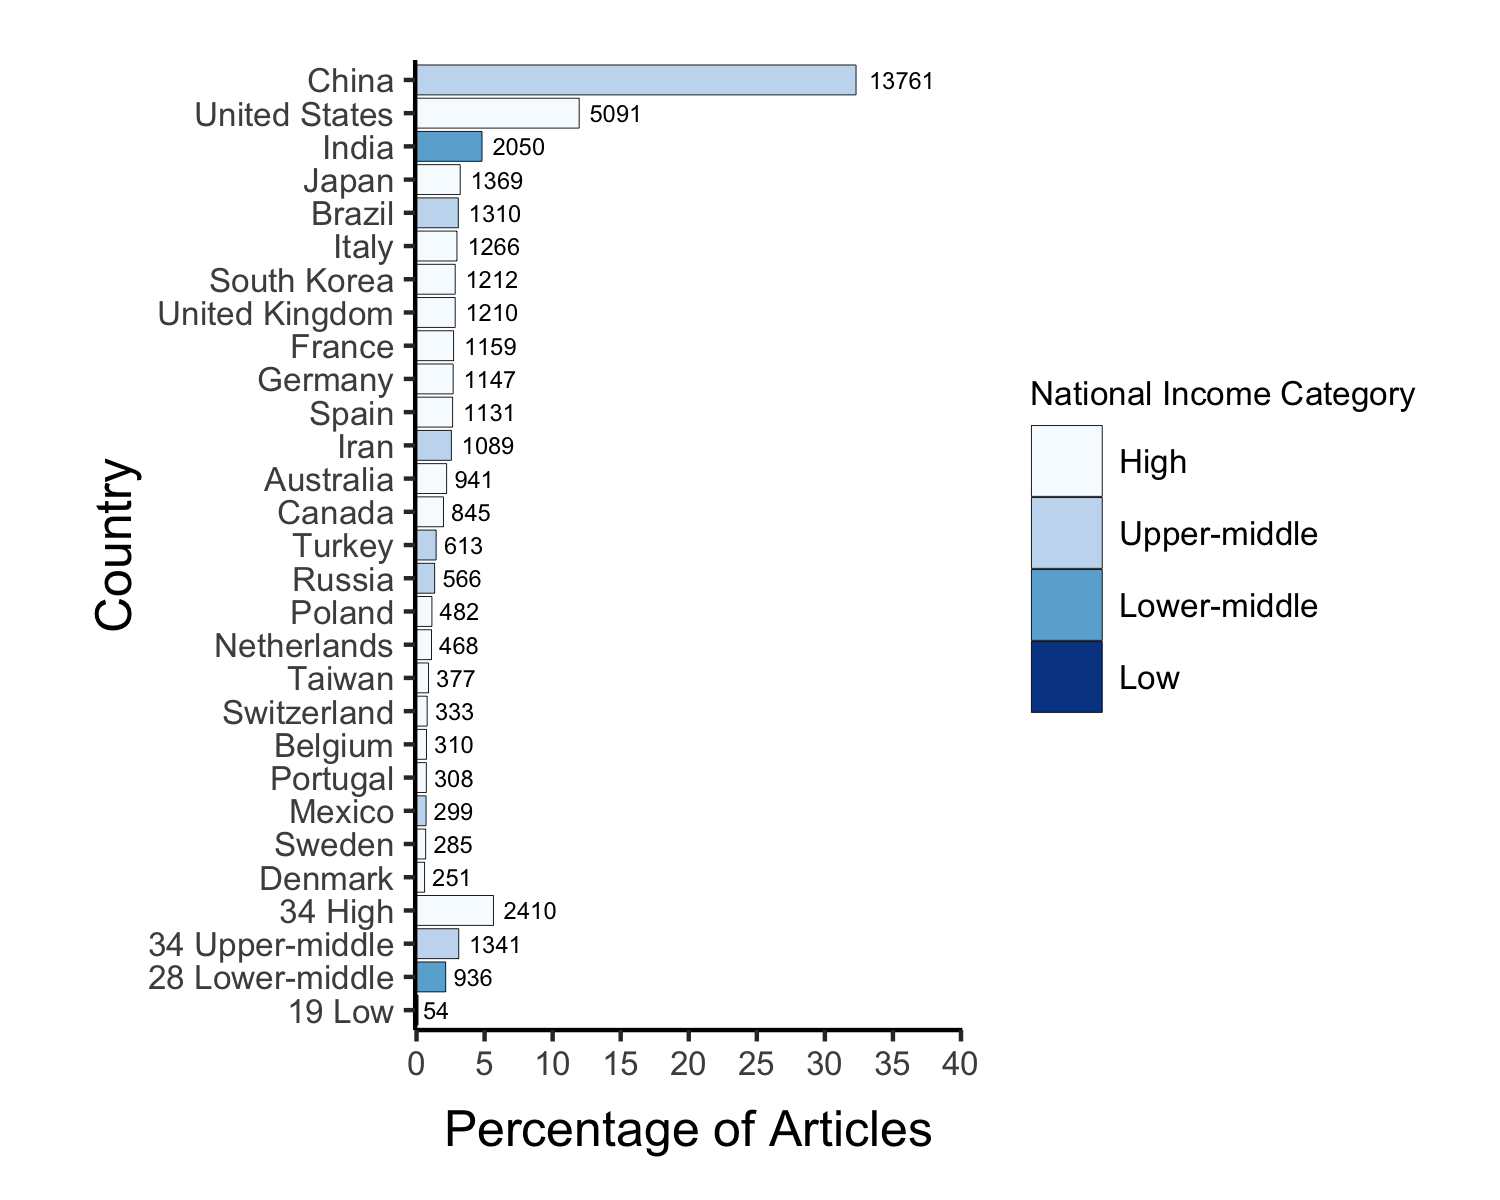
\includegraphics{Smith_etal_APC_ms_files/figure-latex/FigA1-1} 

}

\caption{Percentage of lead authors based in different countries. Includes both paywalled and open access journals. Lead authors includes the authors of sole-authored papers and first authors of co-authored papers. Numbers adjacent to bars are the number of lead authors based in each country.}(\#fig:FigA1)
\end{figure}

\begin{figure}

{\centering 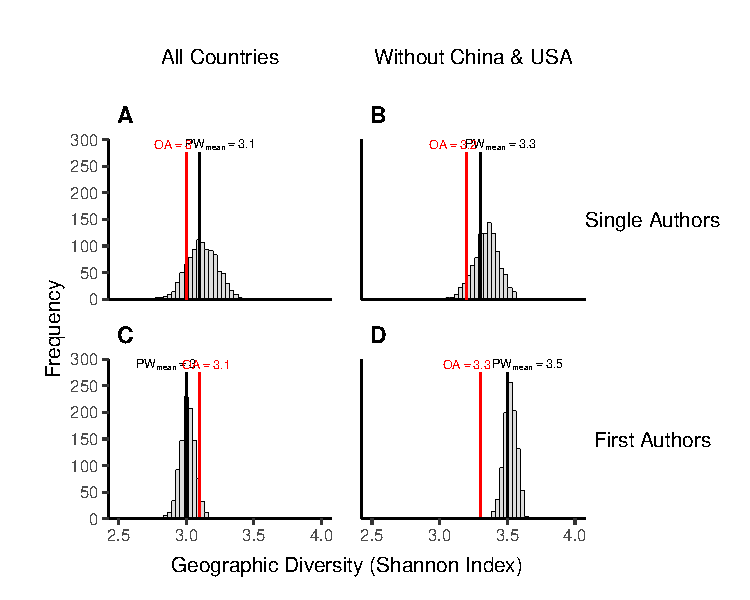
\includegraphics{Smith_etal_APC_ms_files/figure-latex/FigA2-1} 

}

\caption{Author Geographic Diversity (Shannon Index) for pooled Open Access articles (red bar) and 1000 identically sized collections of Paywalled articles selected by bootstrapping. The black line indicates the mean value for the 1000 bootstrap collections.}(\#fig:FigA2)
\end{figure}

\begin{figure}

{\centering 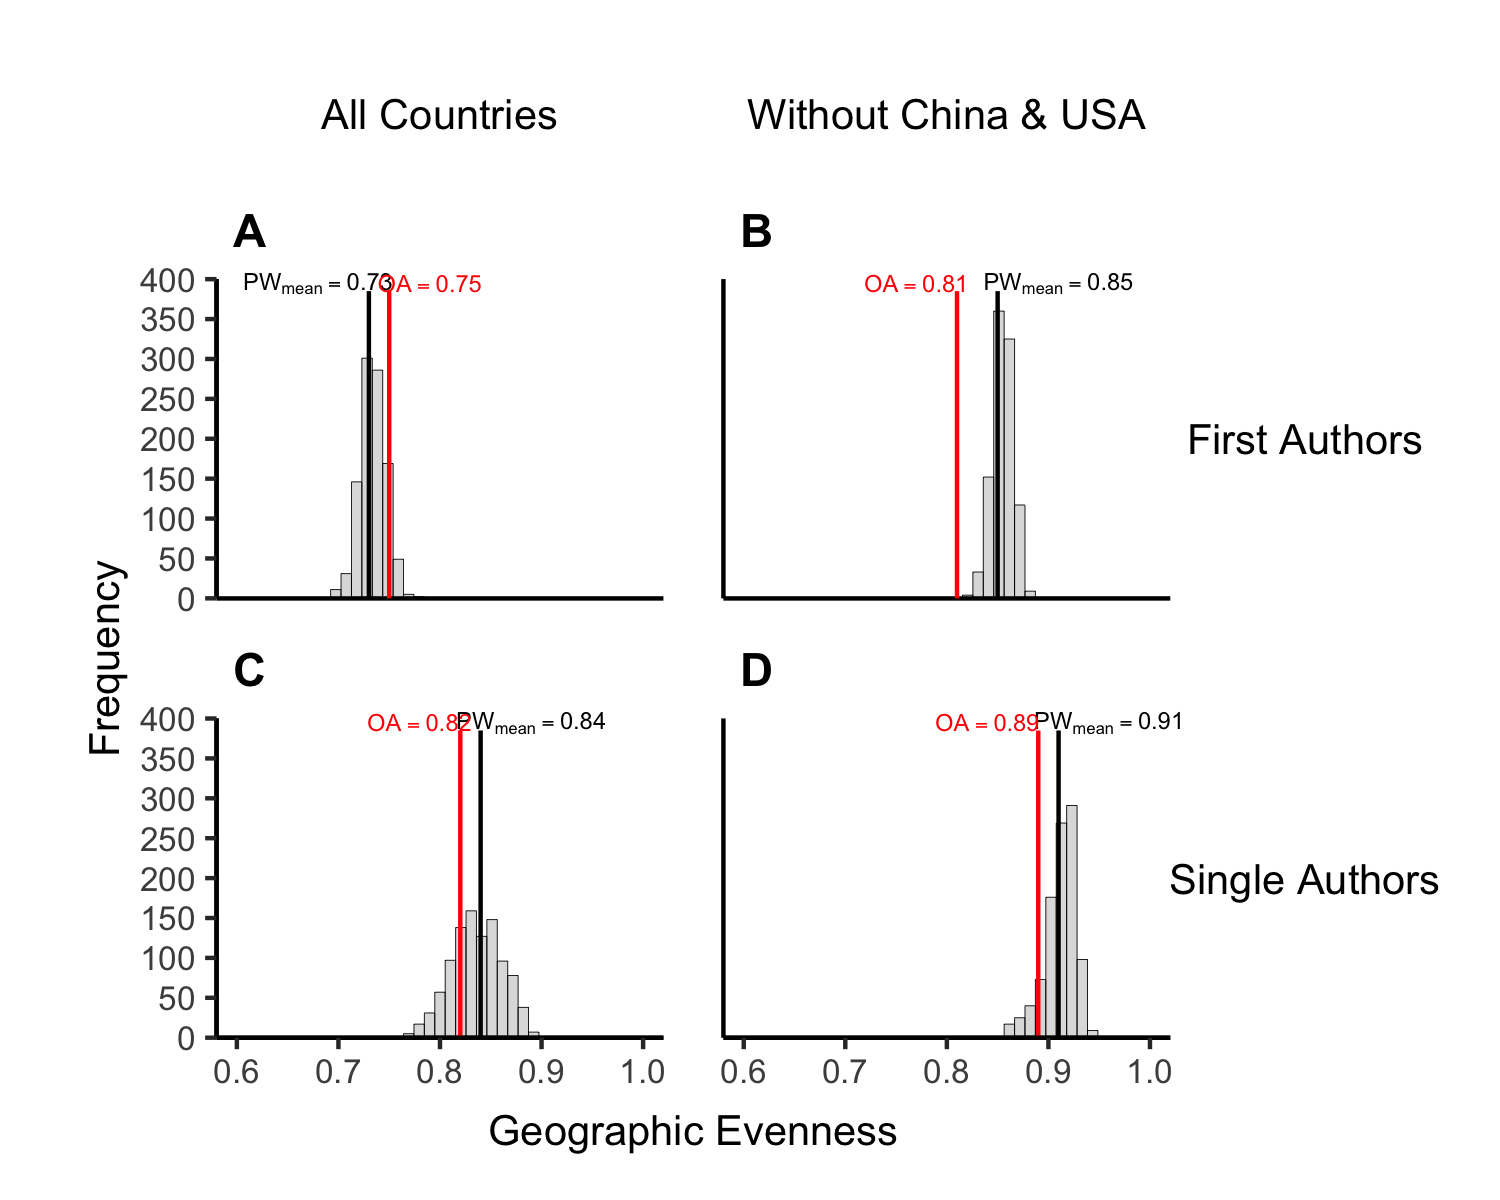
\includegraphics{Smith_etal_APC_ms_files/figure-latex/FigA3-1} 

}

\caption{Proportion of authors of (A) Open Access and (B) Paywalled articles based in different World Bank Lending Groups.}(\#fig:FigA3)
\end{figure}

\newpage
\blandscape
\begin{table}

\caption{(\#tab:AppTable)Countries eligible for APC waivers through Elsevier's 'Research4Life' program by World Bank Global Region and Income Group.}
\resizebox{\linewidth}{!}{
\fontsize{12}{14}\selectfont
\begin{tabular}[t]{ccccc}
\toprule
Region & Income Group & A - 100\% & B - 50\% & no waiver\\
\midrule
South Asia & Low income & Afghanistan, Nepal & - & -\\
 & Middle income & Bangladesh, Bhutan & Maldives, Pakistan, Sri Lanka & India\\
\cline{1-5}
Sub-Saharan Africa & Low income & Benin, Burkina Faso, Burundi & - & -\\
 &  & Central African Republic, Chad, Dem. Repub. Congo, Eritrea & - & -\\
 &  & Ethiopia, Gambia, Guinea, Guinea-Bissau & - & -\\
 &  & Liberia, Madagascar, Malawi, Mali & - & -\\
 &  & Mozambique, Niger, Rwanda, Sierra Leone & - & -\\
 &  & Somalia, South Sudan, Tanzania, Togo & - & -\\
 &  & Uganda & - & -\\
 & Middle income & Angola, Cabo Verde, Cameroon & Botswana, Gabon, Mauritius & South Africa\\
 &  & Comoros, Congo, Equatorial Guinea, Eswatini & Namibia, Nigeria & -\\
 &  & Ghana, Ivory Coast, Kenya, Lesotho & - & -\\
 &  & Mauritania, Sao Tome \& Principe, Senegal, Sudan & - & -\\
 &  & Zambia, Zimbabwe & - & -\\
 & High income & - & Seychelles & -\\
\cline{1-5}
Latin America \& Caribbean & Low income & Haiti & - & -\\
 & Middle income & Belize, Nicaragua & Bolivia, Colombia, Cuba & Argentina, Brazil, Costa Rica\\
 &  & - & Dominica, Ecuador, El Salvador, Grenada & Dominican Republic, Mexico\\
 &  & - & Guatemala, Guyana, Honduras, Jamaica & -\\
 &  & - & Paraguay, Peru, Saint Lucia, Saint Vincent \& the Grenadines & -\\
 &  & - & Suriname, Venezuela & -\\
 & High income & - & Antigua \& Barbuda, Saint Kitts \& Nevis & Aruba, Bahamas, Barbados\\
 &  & - & - & British Virgin Islands, Cayman Islands, Chile, Curaçao\\
 &  & - & - & Panama, Puerto Rico, Saint Martin (FRA), Sint Maarten\\
 &  & - & - & Trinidad \& Tobago, Turks \& Caicos Islands, U.S. Virgin Islands, Uruguay\\
\cline{1-5}
Middle East \& North Africa & Low income & Syrian Arab Republic, Yemen & - & -\\
 & Middle income & Djibouti & Algeria, Egypt, Iraq & Iran, Lebanon\\
 &  & - & Jordan, Libya, Morocco, Tunisia & -\\
 &  & - & West Bank \& Gaza Strip & -\\
 & High income & - & - & Bahrain, Israel, Kuwait\\
 &  & - & - & Malta, Oman, Qatar, Saudi Arabia\\
 &  & - & - & United Arab Emirates\\
\cline{1-5}
E. Asia \& Pacific & Low income & Democratic People’s Republic  Korea & - & -\\
 & Middle income & Cambodia, Fed. States  Micronesia, Kiribati & Fiji, Mongolia, Nauru & American Samoa, China, Indonesia\\
 &  & Laos, Marshall Islands, Myanmar, Papua New Guinea & Vietnam & Malaysia, Philippines, Thailand\\
 &  & Samoa, Solomon Islands, Timor-Leste, Tonga & - & -\\
 &  & Tuvalu, Vanuatu & - & -\\
 & High income & - & Palau & Australia, Brunei, French Polynesia\\
 &  & - & - & Guam, Hong Kong, Japan, Macao\\
 &  & - & - & N. Mariana Islands, New Caledonia, New Zealand, Singapore\\
 &  & - & - & South Korea, Taiwan\\
 &  & Tokelau & Cook Islands, Niue & -\\
\cline{1-5}
Europe \& Central Asia & Low income & Tajikistan & - & -\\
 & Middle income & Kyrgyzstan, Republic  Moldova & Albania, Armenia, Azerbaijan & Bulgaria, Kazakhstan, Romania\\
 &  & - & Belarus, Bosnia \& Herzegovina, Georgia, Kosovo & Russia, Turkey, Turkmenistan\\
 &  & - & Montenegro, North Macedonia, Serbia, Ukraine & -\\
 &  & - & Uzbekistan & -\\
 & High income & - & - & Andorra, Austria, Belgium\\
 &  & - & - & Croatia, Cyprus, Czechia, Denmark\\
 &  & - & - & Estonia, Faroe Islands, Finland, France\\
 &  & - & - & Germany, Gibraltar, Greece, Greenland\\
 &  & - & - & Hungary, Iceland, Ireland, Isle  Man\\
 &  & - & - & Italy, Latvia, Liechtenstein, Lithuania\\
 &  & - & - & -\\
 &  & - & Saint Helena & -\\
\cline{1-5}
North America & High income & - & - & Bermuda, Canada, United States\\
\bottomrule
\end{tabular}}
\end{table}
\elandscape
\end{appendix}
